\documentclass[11pt]{article}
\usepackage[margin=2.54cm]{geometry}
\usepackage[colorlinks,urlcolor=blue]{hyperref}
\usepackage{url}
\usepackage{graphicx}

\title{Classfying Movie Genres With Plot Summaries}
\author{Brian Kimmig, Jesus Zarate}
\date{}

\begin{document}

\maketitle


\section{Introduction}
\label{sec:introduction}

According to Wikipedia a "genre is the term for any category of literature or other forms of art or entertainment" \cite{wiki:genres}. 

Currently, being able to classify what content in language is a hot topic in data science. Something about sentiment analysis. We thought a good way to be introduced to this tool set that allow these analyses was to try and classify writing with pre-made and somewhat objective labels. 

Our first thought was to try to categorized some of the topics in twitter data, but this proved to be hard and not as objective as we would have been responsible for the original categories, which are easily more subjective. 

Using this movie data gives us the opportunity to classify documents with 'correct' answers, allowing us to use a good number of techniques seen in the real world but have more clear cut answers and allow us to make sure that these tools can be used in this manner.

The above may be the key idea?

\section{Data}
\label{sec:data}

We obtained the base of our data from a dataset published on \href{https://www.kaggle.com/deepmatrix/imdb-5000-movie-dataset}{Kaggle}. The dataset contained information on $\sim5000$ movies. We used this dataset for the movie list and the IMDB IDs. With IMDB IDs it is easy to automate gathering the synopses of each movie via GET requests to the \href{https://www.omdbapi.com/}{OMDB API}. The OMDB API allows you to search for movies, and gather information via the title or the IMDB ID. To ensure we get the correct information for every movie we performed GET requests querying with the IMDB ID. 

The OMDB API allows a user to specify the length of the plot summary it returns, with either 'full' or 'short'. We chose to gather the 'full' synopses for every movie we queried.

From the Kaggle data we used the OMDB API to compile title, plot summary, and genres for all $\sim5000$ movies. The data was stored in a JSON file, with each entry (or movie) containing the fields ['title', 'plot', 'genres'].

There were considerably more genres than expected, in total there were 26. Figure \ref{fig:genres} shows every genre and its percent occurrence. In our data, there were genres that occurred less than 1\% of the time, and generally they tended to be more obscure genres. Specifically, the genre 'Game-Show' occurred 0.02\% of the time. Because of the rare genres we decided to limit our genre classification labels to those that occur more often. In the end we settled on a cut of 5\% (shown by the red dotted line in Figure \ref{fig:genres}). This was to ensure that we had captured the major, or most common, genres. The cut of 5\% also allowed us to ensure that every movie had at least 1 label, or genre, associated with it. If the cut was higher, we found that some movies did not have a genre associated with it. We also wanted to avoid throwing away data. 

\begin{figure}[ht]
	\centering
		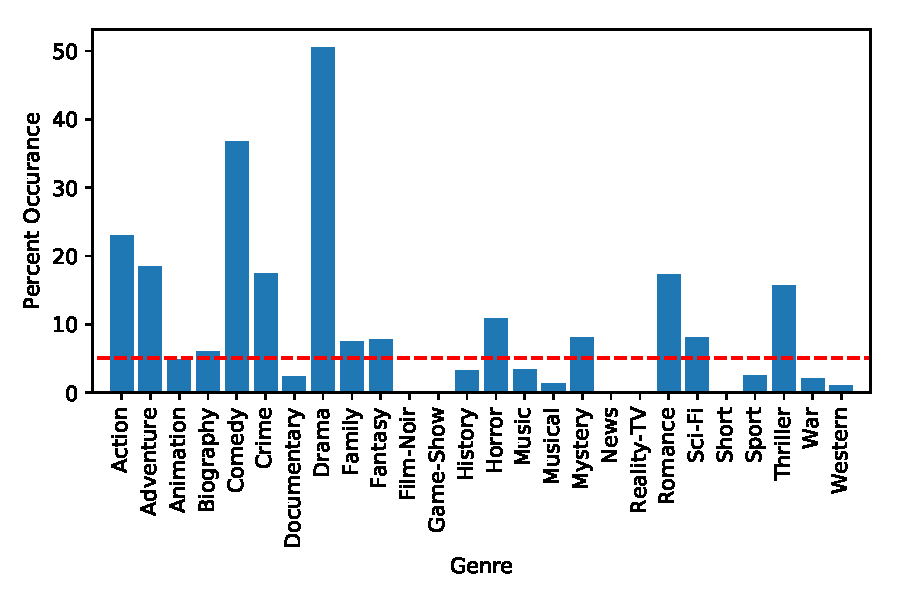
\includegraphics[width=0.75\textwidth]{genres.pdf}
	\caption{The percent occurrence for each genre. The red dotted line represents the cut made to get the list of genres (5\%).}
	\label{fig:genres}
\end{figure}

In the end, with our 5\% cut we ended up with the genres Action, Adventure, Comedy, Crime, Drama, Romance, and Thriller.

The genre labels set up with a one hot encoding. This was done to allow us to easily classify them with either a multi label classifier, or by individually, by column, with other classifiers (discussed further in \S \ref{sec:methods}). Figure \ref{fig:one_hot} shows the genres for every movie in the one hot encoding. A yellow line indicates the movie is associated with that genre, from this we can clearly see that a majority of the movies are associated with the 'Drama' genre.

\begin{figure}[ht]
	\centering
		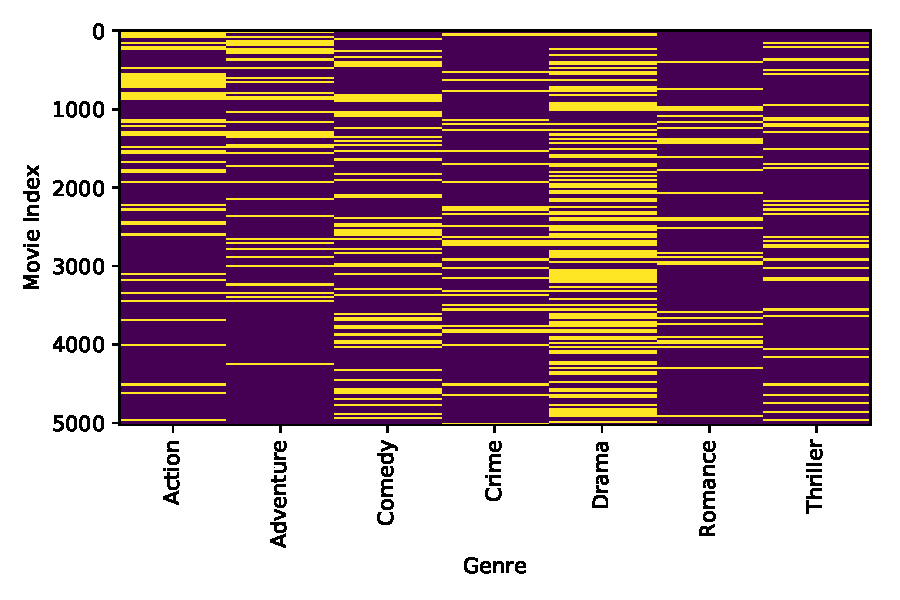
\includegraphics[width=0.75\textwidth]{one_hot_genres.pdf}
	\caption{The one hot encoding of the genres for every movie. Each row represents a movie and a column represents a genre. Yellow indicates the movie has that genres associated with it.}
	\label{fig:one_hot}
\end{figure}

The synopses of the movies live in long strings or documents. We have a list of these that we will processing to create the features that we will then use to build models to classify genres. Extracting features from these documents is the main part of the project and will be discussed \S \ref{sec:methods}.

\section{Key Idea}
\label{sec:key_idea}

\section{Methods and Results}
\label{sec:methods}

\subsection{Term Frequency - Inverse Document Frequency (TF-IDF)}
\label{sec:tfidf}

\subsubsection{Linear Regression}

Classify one genre at a time.

\subsubsection{Logistic Regression}

Classify one genre at a time.

\subsubsection{Random Forrest}

Classify all genres at once.


\subsection{Latent Dirichlet Allocation (LDA)}
\label{sec:lda}

\subsubsection{Linear Regression}

\subsubsection{Logistic Regression}

\subsubsection{Random Forrest}

\subsection{TF-IDF + LDA}
\label{sec:tfidf_lda}

\subsubsection{Linear Regression}

\subsubsection{Logistic Regression}

\subsubsection{Random Forrest}

\section{Discussion}
\label{sec:discussion}

\subsection{Brian's Thoughts}

\subsection{Chuy's Thoughts}

\bibliography{bibliography}{}
\bibliographystyle{plain}

\end{document}

% \begin{table}[h]
% 	\label{tab:genres}
% \begin{center}
% 	\begin{tabular}{| l | l |}
% 		\hline
% 		Genre & \% Occurrence \\
% 		\hline
% 		Action & 23.007\% \\
% 	  \hline  
% 	\end{tabular}
% \end{center}
% 	\caption{}
% \end{table}
